\begin{mybilan}
	\twoCol{
	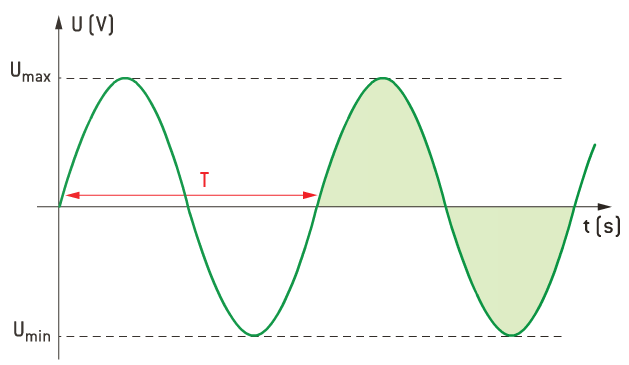
\includegraphics[scale=0.33]{bilan4}	
	\vspace*{1cm}
	\begin{enumerate}
		\item Sur un objet éclairé, la zone qui ne reçoit pas de lumière est l'\kw{ombre propre} de l'objet. 
		\item Sur l'écran la zone qui ne reçoit pas de lumière est l'\kw{ombre portée} de l'objet.
		\item Lorsque l'on change l'orientation de l'objet éclairé, la forme de son ombre portée est modifiée.
	\end{enumerate}}

\end{mybilan}